\documentclass{vldb}

\usepackage{graphicx}
\usepackage{amssymb}
\usepackage{epstopdf}
\usepackage{algorithmic}
\DeclareGraphicsRule{.tif}{png}{.png}{`convert #1 `dirname #1`/`basename #1 .tif`.png}



\def\punto{$\hspace*{\fill}\Box$}
\newcommand{\nop}[1]{}
\newcommand{\tuple}[1]{{\langle#1\rangle}}
\def\lBrack{\lbrack\!\lbrack}
\def\rBrack{\rbrack\!\rbrack}
\newcommand{\Bracks}[1]{\lBrack#1\rBrack}


\newtheorem{theorem}{Theorem}[section]
\newtheorem{proposition}[theorem]{Proposition}
\newtheorem{example}[theorem]{Example}
\newtheorem{remark}[theorem]{Remark}
\newtheorem{todo}[theorem]{ToDo}
\newtheorem{algorithm}[theorem]{Algorithm}

\numberofauthors{3}
\title{Cumulus: Combining Periodic and Eventual Consistency (in the cloud)}
\author{
\alignauthor
Oliver Kennedy\\
  \affaddr{Cornell University}
  \affaddr{okennedy@cs.cornell.edu}
\alignauthor
Yanif Ahmad\\
  \affaddr{Cornell University}
  \affaddr{yanif@cs.cornell.edu}
\alignauthor
Christoph Koch\\
  \affaddr{Cornell University}
  \affaddr{koch@cs.cornell.edu}
}
\date{}
\toappear{}

\begin{document}
\maketitle

\begin{abstract}

\end{abstract}

\section{Introduction}

Recent years have seen the beginning of a paradigm shift in data management research from incrementally improving decades-old database technology to questioning established architectures  and creating fundamentally different, more lightweight systems that are often domain-specific (e.g.,
%\cite{DBLP:conf/cidr/KerstenM05,DBLP:conf/vldb/StonebrakerMAHHH07}
\cite{DBLP:conf/vldb/StonebrakerMAHHH07,DBLP:journals/pvldb/KallmanKNPRZJMSZHA08}).

Part of the impetus for this change was given by potential users such as scientists and the builders of large-scale Web sites and services such as Google, Amazon, and Ebay, who have a need for data management systems but have found current databases not to scale to their needs. One can observe a trend to disregard database contributions in these communities \cite{dbcolumn, DBLP:conf/sigmod/PavloPRADMS09}, and to build lightweight systems based on robust technologies mostly pioneered by the operating systems and distributed systems communities, such as large scale file systems, key-value stores, and map-reduce \cite{DBLP:journals/cacm/DeanG08, DBLP:journals/tocs/ChangDGHWBCFG08}. Further impetus has resulted from the current need to develop data management technology for multicore and cloud computing.

There is a recent tendency among pundits outside the database community to contest the need for powerful queries, and to think of key-value stores -- with only the power to look up data by keys -- as (much more efficient) database query engines.

However, expressive query languages such as SQL continue to act as an important intermediary between users and more complex data-processing tasks.  Alas, we do not know how to process SQL queries on updateable data using a system as lightweight as a key-value store.

This paper contributes a fundamental and versatile building block for enabling new, more lightweight and nimble data processing systems based on SQL aggregation queries.  Cumulus is a thin execution layer that lives above generic key-value stores and can efficiently process a wide range of incremental view queries.  The query results are stored in the key-value store itself, as ordinary data. 

Cumulus is built around a novel hybrid consistency execution framework.  Like most cloud data management systems, Cumulus achieves low latencies by retreating to the realm of eventual consistency.  However, unlike most eventual consistency systems, Cumulus' runtime periodically generates consistent snapshots as a side effect of its normal operation.  The result is a system that can be employed side-by-side by both applications that require low latency and applications that require strong consistency.

We believe that our contribution constitutes an important step towards achieving the apparent contradiction in terms of executing complex aggregation queries on updateable data using little more than a key-value store.

At the heart of our approach is M3, a trigger-based vector processing language.  M3 can either be written directly by hand or translated from SQL with DBToaster\cite{1687592}, an aggressive recursive incremental view maintenence compiler.  In most traditional database query processors, the basic building blocks of queries are large-grained operators such as joins.  Conversely, a large class of SQL aggregation queries can be compiled down to very simple message passing programs that incrementally maintain materialized views of the queries.

These message passing programs keep a hierarchy of map data structures (which may be served out of a key-value store) up to date. They can share computation in the case that multiple aggregation queries (e.g., a data cube \cite{datacube}) need to be maintained.  Most importantly, though, these message passing programs can be massively parallelized to the degree that the updating of each single result aggregate value can be done in constant time on normal off-the-shelf computers\footnote{Note that since there are
usually many more aggregate values to maintain than there are processors,
this does not mean that each update is processed in constant time.}.

Our main technical contributions are as follows:
\begin{itemize}
\item We present M3, a massively parallizable language for message passing programs that can be used to incrementally maintain SQL aggregation queries.
\item We present Cumulus, a lightweight realtime exact online aggregation system that integrates seamlessly with generic key-value stores. 
\item We describe three different approaches to managing the consistency of query results: Centralized Target Aggregation, Centralized Source Aggregation, and Hybrid Consistency Source Aggregation.  We demonstrate how the last of these techniques simultaneously produces low-latency eventually consistent results as well as periodic consistent snapshots.
\item We show evidence for the scalability of our approach by examining the performance of Cumulus on examples drawn from the TPC-H benchmark\cite{tpch2008}
\end{itemize}


\section{The M3 Update Calculus}
Cumulus is built around M3, a trigger-based language closely related to Relational Calculus.  The basic datatype in M3 is the map, a mapping from vectors of keys to numeric values, or entries.  An M3 program consists of a set of triggers of the form
\[
\mbox{{\tt on <R>($\vec x \vec y$) \{ $s_1$; $\dots$; $s_k$ \}}}
\]
where {\tt <R>} is an event parametrized by a set of \textit{event variables} $\vec x \vec y$.  For example, for an M3 program that incrementally computes the results of a SQL query, an event would be a user inserting a row into a relation.  Each event triggers the evaluation of a list of statements $s_i$ each of which updates zero or more entries in a single map.
\[
\mbox{$m[\vec{x}\vec{z}]$ {\tt +=} $t(\vec x \vec y \vec z)$}
\]
Statements are comprised of a reference to a map entry on the left-hand side, and a right-hand side consisting of a term: a monomial algebraic expression over constants, variables, and map lookups parametrized by variables.  A simplified version of M3 that will be used in this paper is presented in Figure \ref{fig:m3_defn}

Two types of variables appear in M3 statements: event variables $\vec x, \vec y$ as defined above, and \textit{loop variables} $\vec z$.  Loop variables draw their domains from the right-hand side maps that they parametrize.  For example, consider the trigger:
\[
\mbox{\texttt{ON R(A) \{ m1[B] += m2[A,B] \}}}
\]
When Event \texttt{R(A)} occurs, every value \texttt{m1[B]} will be incremented by the corresponding \texttt{m2[A,B]}\footnote{Because all operations in M3 are increments, default values are required for each map entry.  In the simplified version of M3 that we describe here, the default value is always 0.}.  In effect, this is a multidimensional vector operation where the \textit{slice} of map \texttt{m2} with first parameter equal to \texttt{A} is extracted and used to increment \texttt{m1}.  Because the right hand side must be a monomial, only values of \texttt{B} for which \texttt{m2[A,B]} is nonzero can affect \texttt{m1}.  These values form the \textit{domain} of loop variable \texttt{B}.  Note that the domains of two loop variables may be linked if they appear as parameters to the same map.

%The domains of two variables may be linked.  For example, consider the trigger:
%\[
%\mbox{\texttt{ON R() \{ m1[B,C] += B \cdot m2[B,C] \}}}
%\]
%The domain of \texttt{C} is dependent on the value of \texttt{B} and visa versa.

M3 provides two consistency guarantees for programs:
\begin{itemize}
\item Triggers execute atomically with respect to each other.
\item Statements within a trigger execute in order.
\end{itemize}
These guarantees are equivalent to serializable consistency, where each event constitutes a transaction.


\subsection{Restricted M3}

For the purposes of this paper, we restrict ourselves to a limited, fully incremental version of M3.  
\begin{itemize}
\item \textit{All loop variables appear on both sides of a statement.}  The natural implication of a loop variable appearing only on the right-hand side is as a sum aggregate over the variable.  In restricted M3, this aggregate can be computed incrementally by maintaining an additional map with one fewer key.
\item \textit{All loop variables appear as a parameter to exactly one right-hand side map.}  A loop variable that appears in two right-hand side maps is effectively a join between the maps.  In restricted M3, joins are computed incrementally using event variables.  Note that this restriction results in each loop variable's domain being defined by exactly one map.
\item \textit{Terms do not contain conditions.}  Unrestricted M3 supports conditioned non-incremental aggregates.
\item \textit{Map data dependencies are acyclic, even across multiple events.} A non-recursive SQL query be represented as an M3 program with no cyclic data dependencies.  Restricted M3 does not attempt to support recursive queries.
\end{itemize}

Distributing unrestricted M3 is beyond the scope of this paper.  As shown in \cite{dbtoaster-pods}, this restricted form of M3 remains powerful enough to express any non-recursive SQL count or sum aggregate query without inequalities.  

\begin{example}
Consider the following query over a TPC-H-like schema.
\begin{verbatim}
SELECT   c.nation, l.part
         SUM(o.discount * l.price)
FROM     CUSTOMERS c, ORDERS o, LINEITEMS l
WHERE    c.cid = o.cid AND o.oid = l.oid
GROUP BY c.nation, l.part
\end{verbatim}

This query can be implemented in streaming form as the following M3 program\footnote{Only insertion triggers are shown.  Deletion triggers are identical except for a multiplier of -1 applied to each right-hand side.}.
\begin{verbatim}
ON +LINEITEMS(OID,PRICE,PART) DO {
 q[PART,NATION] += m1[OID,NATION] * PRICE;
 m2[CID,PART]   += m3[CID,OID] * PRICE;
 m4[OID,PART]   += PRICE }
ON +ORDERS(CID,OID,DISCOUNT) DO {
 q[PART,NATION] += DISCOUNT * m4[OID,PART] * 
                     m5[CID,NATION];
 m1[OID,NATION] += DISCOUNT * m5[CID,NATION];
 m2[CID,PART]   += DISCOUNT * m4[OID,PART];
 m3[CID,OID]    += DISCOUNT }
ON +CUSTOMERS(CID,NATION): 
 q[PART,NATION] += m2[CID,PART];
 m1[OID,NATION] += m3[CID,OID];
 m5[CID,NATION] += 1 }
\end{verbatim}
Here, the map \texttt{q} represents the query result, while other maps represent intermediate subqueries.  For example, \texttt{m2} represents 
\begin{verbatim}
SELECT   o.cid, o.priority, 
         SUM(o.discount * l.price) 
FROM     ORDERS o, LINEITEMS l
WHERE    o.oid = l.oid
GROUP BY o.cid, o.priority
\end{verbatim}
To see how loop variables are not required for an incremental join, note the three lines that update the result map \texttt{q}.  Each line incrementally updates the full join result by joining only with the tuple being inserted.
\end{example}

\begin{figure}
\begin{center}
{\small
\begin{eqnarray*}
PROGRAM & := & TRIGGER; TRIGGER; \ldots\\
TRIGGER & := & \textbf{ON}\ \left <EVENT\right>\ ( evt\_var_1, evt\_var_2, \ldots )\\ & & \textbf{DO}\ \{ STMT; STMT; \ldots\}\\
STMT & := & map_{target}[VAL_{1}, \ldots]\ \textbf{+=}\ EXPR\\
EXPR & := & map_{k}[VAL_{a}, \ldots]\ |\ VAL\ |\\&& EXPR\ *\ EXPR\ |\\&& \textbf{IF}\ EXPR\ CMP\ EXPR\\&& \textbf{THEN}\ EXPR\ \textbf{ELSE 0}\\
VAL & := & evt\_var_{n}\ |\ loop\_var_{m}\ |\ constant\\
CMP & := & =\ |\ <\ |\ <=
\end{eqnarray*}}
\caption{A restricted subset of M3}
\label{fig:m3_defn}
\end{center}
\end{figure}



\section{Centralized Consistency}

As all statements in M3 are effectively vector operations over maps, the language is extremely amenable to distribution.  Cumulus distributes both data and processing over a cluster of \textit{nodes}, each using BerkleyDB(TODO: Cite??) as a local shared-nothing key-value store for map entries\footnote{Though Cumulus uses the secondary indexing and iteration capabilities of BerkleyDB, both features can be built into or atop any key-value store.}.

All data in Cumulus is stored as part of a map - either as the value of a map entry, or as one of the entry's keys.  A map is horizontally partitioned into one or more \textit{map segments} along any or all of its keys, and each segment is stored on one or more nodes in the cluster.

Nodes interact with the outside world via one or more \textit{coordinators}.  Event sources (eg., ticker feeds, sensors, static files, relational databases, or even other M3 programs) send events to the coordinator(s).  The coordinator optionally appends the event to a redo log, tags it with a timestamp, and dispatches it to the cluster of nodes for processing.  The overall design of Cumulus is illustrated in Figure \ref{fig:architecture}.

\begin{figure}
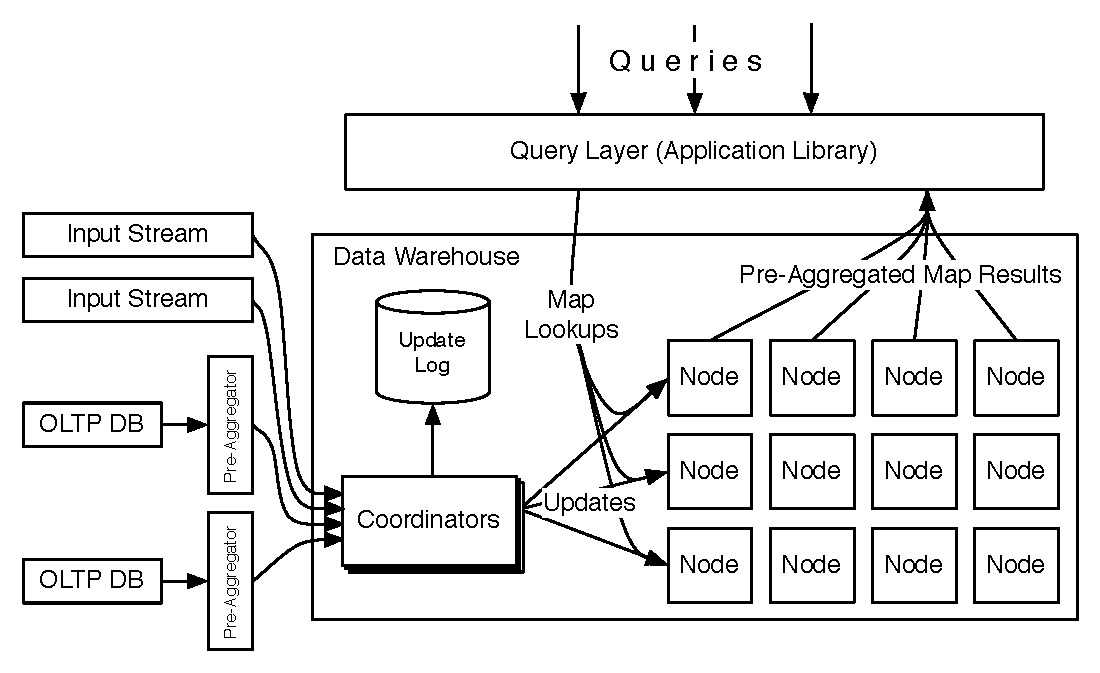
\includegraphics[width=3in]{graphics/Architecture.pdf}
\caption{The Cumulus Architecture}
\label{fig:architecture}
\end{figure}

External applications access map nodes directly, using a mapping of map segments to nodes, or \textit{layout} obtained from the coordinator.  With the layout, the application fetches desired map values directly from nodes storing the values.  Cumulus provides library methods for doing so, described in Figure \ref{fig:queryapi}.  The API allows the client to indicate that a sum, min, or max aggregate is required, so that nodes can pre-aggregate matching values locally to reduce messaging overhead.

\begin{figure}
\begin{algorithmic}
\STATE \textbf{READ\_SLICE}(map, $key_1$, $key_2$, \ldots) 
\end{algorithmic}
\hspace*{0.2in}\parbox[b]{3in}{Read the current version of a slice of a map; Null keys are treated as wildcards. All matching nonzero entries are returned.}
\begin{algorithmic}
\STATE \textbf{READ\_SUM}(map, $key_1$, $key_2$, \ldots)
\STATE \textbf{READ\_MIN}(map, $key_1$, $key_2$, \ldots)
\STATE \textbf{READ\_MAX}(map, $key_1$, $key_2$, \ldots)
\end{algorithmic}
\hspace*{0.2in}\parbox[b]{3in}{As READ\_SLICE but preaggregate values at the node if possible.  Null keys are treated as wildcards. The sum, min, max, etc\ldots of nonzero matching entries is returned.}
\begin{algorithmic}
\STATE \textbf{READ\_STABLE}(map, agg\_type, $key_1$, $key_2$, \ldots)
\end{algorithmic}
\hspace*{0.2in}\parbox[b]{3in}{As READ\_SLICE, but guarantees a self-consistent result when using eventual consistency (See Section \ref{sec:eventualconsistency}).  Returns the most recent consistent snapshot of all matching nonzero entries with optional pre-aggregation.}
\caption{Cumulus' Query API}
\label{fig:queryapi}
\end{figure}

\subsection{Distributing M3}
We consider two approaches to distributing data processing and data storage across nodes in the cluster in order to minimize network overheads.  
\begin{enumerate}
\item Co-locate the processing of an M3 statement with the node storing the left-hand side map - that is, the map being updated. We refer to this as \textit{target aggregation}.
\item Co-locate the right-hand side maps of an M3 statement on the same node that processes the statement.  We refer to this as \textit{source aggregation}.
\end{enumerate}
As we will show, these questions are also intricately linked to the primary challenge of distributing M3: ensuring serializably consistent execution. 

Throughout the following sections, we will assume that each node is fully aware of the data layout.  The generation and dynamic management of layouts is beyond the scope of this paper.

\subsection{Target Aggregation}
In target aggregation, M3 statements are evaluated at the node that will store the results.  Data appearing on the right-hand side of the statement is sent to this node for delta computation.  

\begin{example}
Consider the following M3 statement with maps \texttt{m1} and \texttt{m5}, each partitioned only on attribute N.
\begin{verbatim}
ON +ORDERS(C,O,D) DO { m1[O,N] += D * m5[C,N] }
\end{verbatim}
When event \texttt{+ORDERS} occurs, each node storing a segment of \texttt{m5} will send each value in its segment to the node storing the corresponding segment of \texttt{m1}.  If the partition boundaries of \texttt{m1} and \texttt{m5} are identical, each \texttt{m5} node will send its entire segment to exactly one \texttt{m1} node.  This process is illustrated in Figure \ref{fig:messagepassing}a.  Note that If the same node stores each pair of corresponding \texttt{m1} and \texttt{m5} partitions, no actual data transmission occurs.  
\end{example}

Even if \texttt{m5} is also partitioned over \texttt{O}, each \texttt{+ORDERS} event updates only one map segment per \texttt{B} value; A node storing a segment of \texttt{m5} is still only required to send the segment to one \texttt{m1} node.  However, there are situations where multicast is required.  

\begin{example}
Consider the following statement:
\begin{verbatim}
ON +ORDERS(C,O,D) DO { q[P,N] += D * m4[O,P] 
                                   * m5[C,N] }
\end{verbatim}
Let \texttt{q} have 10 partitions in a grid pattern, with the domain of \texttt{P} split in half and \texttt{N} split into 5 parts.  Let \texttt{m4} and \texttt{m5} use the same partitioning scheme (with 2 and 5 partitions, respectively).  In this instance, when an \texttt{ORDERS} event occurs, each \texttt{m4} node sends its segment to each of the corresponding 5 \texttt{q} nodes, while each \texttt{m5} node will send its segment to each of the corresponding 2 \texttt{q} nodes.  This process is illustrated in Figure \ref{fig:messagepassing}b. 

If a right-hand side map contains an event variable, only a subset, or slice of the map is sent.  For example:
\begin{verbatim}
ON +ORDERS(C,O,D) DO { m1[O,N] += D * m5[C,N] }
\end{verbatim}
In this instance, only the slice \texttt{m5'[N] = m5[C,N]} is sent.
\end{example}

\begin{figure}
\begin{center}
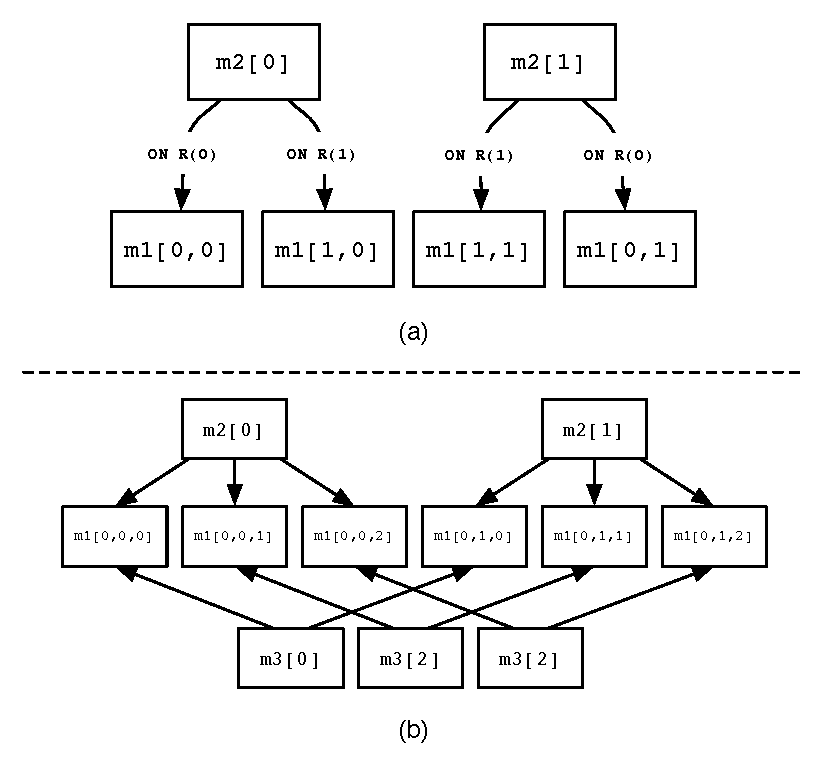
\includegraphics[width=3in]{graphics/message_passing}
\caption{Messages sent during evaluation of a single M3 statement in target aggregation, assuming a uniform partitioning scheme.  (a) The statement \texttt{on~R(A)~:~m1[A,B]~+=~m2[B]} (b) The statement \texttt{on~R(A)~:~m1[A,B,C]~+=~m2[B]*m3[C]} }
\label{fig:messagepassing}
\end{center}
\end{figure}

\subsection{One Coordinator}
The simplest way to provide M3's serializable execution guarantees is to route all events through a centralized coordinator.  Though centralizing creates a scalability bottleneck, the central coordinator's task is straightforward event serialization and dissemination.  The task of dissemination is further simplified by building a distribution tree over the nodes themselves.

As a query is loaded, each node precomputes a table of directives from the M3 program and the data layout.  This table indicates for each class of event (where class is defined by the partitioning scheme), which of the node's map segments will be modified (ie, those that appear on the left-hand side of a triggered statement), and which segments will be read from (right-hand side).  The construction algorithm is shown in Figure \ref{fig:directiveconstruction}.

\begin{figure}
\begin{algorithmic}[1]
\FORALL{Event Variable $V$ in Statement $S$}
  \STATE $partitions[V]$ = 1;
  \FORALL{Map $M \in S$ with $V$ as a key}
    \STATE \COMMENT {Run once for each occurrence of V in S as a key}
    \STATE $C =$ \# of partitions of $M$ on the $V$ axis.
    \STATE $partitions[V] =$ compute\_lcm($partitions[V]$, $C$)
  \ENDFOR
\ENDFOR
\FOR{$P \in \mathbb N^{|partitions|}$ with $0 \leq P_V < partitions[V]$}
  \STATE $Directive[P] = \{\}$
  \FORALL{Map $M \in$ right\_hand\_side($S$)}
    \FORALL{Event Variable $V$ in $M$}
      \STATE $C =$ \# of partitions of $M$ on the $V$ axis.
      \STATE $slice[V] = C\cdot\frac{P}{partitions[V]}$
    \ENDFOR
    \STATE \COMMENT{Note that the slice may have multiple owners}
    \STATE $Dir[P] +=$ \{\textbf{read $M$ from} owner($M, slice$)\}
  \ENDFOR
  \STATE $M = target\_map(S)$
  \FORALL{Event Variable $V$ in $M$}
    \STATE $C =$ \# of partitions of $M$ on the $V$ axis.
    \STATE $slice[V] = C\cdot\frac{P}{partitions[V]}$
  \ENDFOR
  \STATE $Dir[P] +=$ \{\textbf{write $M$ to} owner($M, slice$)\}
\ENDFOR
\STATE \textbf{return} $Dir$
\end{algorithmic}
\caption{The directive table construction algorithm.}
\label{fig:directiveconstruction}
\end{figure}

The coordinator first assigns a version number to each event.  Then, when a node receives an event from the distribution tree, it consults the directive table for the appropriate read and write operations to perform.  

Write operations are deferred until all prior writes on the map have been completed, and all slices appearing on the right hand side of the update statement have been received.  

Similarly, read operations block until all write operations on the map pending at the time of the event are complete.  Upon completion of the last prior write, the source node gathers the required slices, and sends them to the corresponding destination nodes.  Note that the even empty slices must be sent; the destination node needs to hear from all source nodes in order to proceed with its write.

\subsection{Source Aggregation}
Instead of processing updates at the node where the result will be stored, precompilation allows Cumulus to ensure that all data necessary to process a statement is co-located. In this scheme, each map segment is stilly processed at a specific node.  Rather than storing the results locally, a replica of the map segment is created at each node that reads from the segment.  

Consistency is maintained in the same way as in Target Aggregation.  When an event occurs, each node identifies which local maps might be updated as a consequence.  As before, writes are deferred until all input maps have been updated.  Also, as before, writes are always sent across the wire, even if no updates actually occur.  

When discussing source aggregation, we assume without loss of generality that each node processes updates for exactly one map, and refer to maps and nodes interchangeably.  Where the distinction is relevant, maps are indicated with \texttt{fixed width font}.

\section{Decentralized Consistency}
Both target and source aggregation attempt to enforce serializable consistency.  This introduce delays into update processing, and also requires the use of ``empty'' messages.  Worse still, the centralized coordinator creates a single point of failure and a scalability bottleneck.  

The M3 language affords Cumulus a critical benefit: map data is changed only by offset.  Thus, the messaging overhead of an undo operation is equivalent to that of a write.  Cumulus exploits the low undo overhead in order to achieve a processing model that simultaneously generates both low-latency eventual consistency outputs and periodic consistent snapshots.  

\subsection{Eventual Consistency}
\label{sec:eventualconsistency}
In the eventual consistency approach, there are multiple coordinators, each with a numeric identifier.  Coordinators maintain a loosely synchronized clock between themselves, and use it to define epoch boundaries.  Synchronized epoch transitions are not required.  However, tighter inter-coordinator epoch transitions result in a more efficient system.  This is discussed further below.

By decentralizing, each coordinator is freed to do additional work to minimize network usage.  Each coordinator maintains a dispatch table, similar to the directive table used by the nodes under centralized consistency.  The table maps  partitions of each event's parameter space to the set of nodes required to process the partition.  When an event occurs, only these nodes are notified.

Each event is sent to a coordinator, where it is assigned a version identifier consisting of the three-tuple \texttt{\{VersionID, CoordinatorID, EpochID\}}.  Here, the version identifier is a unique identifier, monotonically increasing at the coordinator within a given epoch.  This three-tuple is enough to create a total ordering over all version identifiers by sorting by epoch, coordinator, and then version.  An ordering over map updates can be created by extending the three-tuple with the ordering of the M3 statements.  

Nodes follow the Source Aggregation approach, but instead of deferring writes, send them as soon as possible.  For improved efficiency, this includes a small buffer period.  Writes are recorded in a short-term log, along with the event and statement that produced them.  The value of the delta is computed immediately based on the source maps' current values, excluding deltas tagged with later versions.  The resultant delta is sent immediately.  

When a node receives a map delta, it identifies all earlier updates in its history.  It then determines which of these updates are affected by the incoming delta, computes the new delta, and sends the difference between the deltas.  Pseudocode for this process is presented in Figure \ref{fig:eventualconsistency}.

\begin{figure}
ON Event $R(\vec X)$ with version $V$
\begin{algorithmic}[1]
\FORALL{Statement $S_i$ Triggered By $R(\vec X)$}
	\STATE $target =$ target\_map($S_i$)
	\STATE $\delta =$ compute($S_i$, $\vec X$, $V$)
	\IF{$\delta \neq \emptyset$}
    \STATE send\_push($target$, $\vec X$, $\delta$, $V \circ i$)
  \ENDIF
	\STATE $history[V\circ i] = \{S_i, \vec X, \delta\}$ 
\ENDFOR
\end{algorithmic}
\ \\
ON Push($target$, $\vec X$, $\delta$, $V$)
\begin{algorithmic}[1]
\FORALL{Key $\vec E \in \delta$}
  \STATE sorted\_insert($target[\vec E]$, $V$, $\delta$)
  \COMMENT {Map entries are stored as a list of deltas, sorted by version}
\ENDFOR
\FORALL{$\{S, \vec X', \delta'\} \in history[V']$ with $V' > V$}
	\IF{$S$ read from $target$}
		\STATE $\delta_{new} =$ compute($S$, $\vec X'$, $V'$) - $\delta$
    \IF{$\delta_{new} \neq \emptyset$}
      \STATE send\_push(target\_map($S$), $\vec X'$, $\delta_{new}$, $V'$)
    \ENDIF
	\ENDIF
\ENDFOR
\end{algorithmic}
\ \\
ON compute($S$, $\vec X$, $V$)
\begin{algorithmic}[1]
\STATE $slice = \{[] \rightarrow 1\}$
\STATE \COMMENT {We assume there is at least one term.  Terms may be numerics (treated as $\{[]\rightarrow \#\}$) or map accesses.}
\FORALL{Term $T_i[\vec Y] \in $ terms($S$)}
  \STATE \COMMENT {$\times$ and $\bowtie$ are the cross product and natural join}
  \STATE $term\_slice[\vec Y] = \sum_{\vec Y \bowtie \vec X; V' \leq V} T_i[\vec Y][V']$
  \STATE $slice = slice \times term\_slice$
\ENDFOR
\STATE $\delta =$ project($slice$, keys(target\_map($S$)))
\STATE \textbf{return} filter(delete $[*]\rightarrow 0$, $\delta$)
\end{algorithmic}
\caption{The Eventual Consistency Update Algorithm (simplified).}
\label{fig:eventualconsistency}
\end{figure}

\begin{figure}
\begin{center}
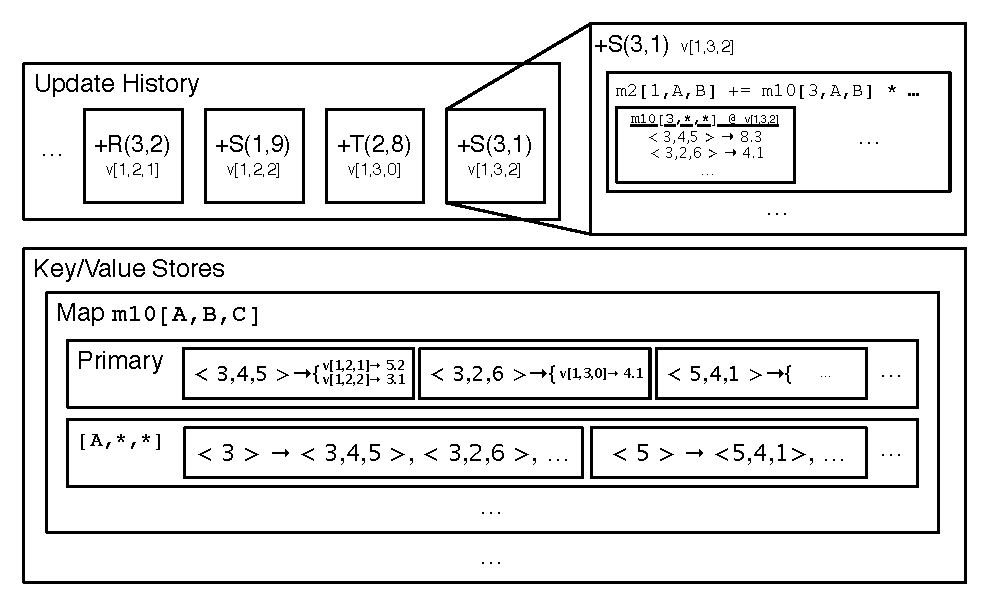
\includegraphics[width=3.4in]{graphics/Datastructures}
\caption{Datastructures used at each node.  The update history stores updates since the last garbage collection together with a cache of precomputed map values at a particular version number.  One key-value store is used for each map.  If the key-value store does not support secondary indices, the same effect may be achieved by using an additional store for each secondary index required.  The key-value store maintains one delta for each version in which a map entry entry was modified.}
\label{fig:datastructures}
\end{center}
\end{figure}

The values stored in a map may not be correct at any given moment.  For example, consider the partial M3 program:
\begin{verbatim}
ON R(A,B): m1[] += m2[A]
           m2[A] += m3[B]
\end{verbatim}
This fragment of the program is deployed with no segmentation on a 2 node system.  Node 1 stores m2 and processes updates to m1, while Node 2 stores m3 and processes updates to m2.  

In this scenario, two subsequent R events with identical A parameters are dispatched by the same coordinator nearly simultaneously.  Both nodes process the necessary updates to m1 and m2 respectively.  However, while node 1 is processing the second event, it does not have the value of m2 updated by the first event.  The result is a value of m1 that is incorrect.  However, when the updated value of m2 is received, Node 1 can overwrite the corresponding version of m1.  

This process maintains an eventually consistent version of all maps.  The value of the maps may not be consistent at any given moment, but the error is limited to values that have not fully propagated through the system.  Thus, if the system quiesces, maps will return to consistency.

\subsection{Data Dependencies}
Event $E_2$ is dependent on event $E_1$ if $E_2$ has a later timestamp, and reads reads from a map entry that $E_1$ writes to\footnote{Note that since M3 statements manipulate entire maps, dependencies at the entry granularity are data-dependent}.  Concretely, $E_2$ is dependent on $E_1$ if a non-zero entry appears in the intersection between a slice appearing on the right-hand side of a statement issued by $E_2$, and a left-hand slice from $E_1$.  

An unfulfilled dependency occurs at a node $N$ if an event $E_2$ depends on event $E_1$, but $E_1$'s deltas do not arrive at node $N$ until after $N$ has sent out the delta it produces for $E_2$.  Unfulfilled dependencies are handled by sending out a corrective delta, as described above.  However, the corrective delta may be the source of another unfulfilled dependency at the target node if the target has already processed an event with a timestamp after $E_2$'s.  We refer to such an event as a cascade.

We can examine the effects of a cascade by considering the dataflow hypergraph of an M3 program, such as the one in Figure \ref{fig:dataflow}.  In a dataflow graph, each node represents one map and each hyperedge represents a statement.  Hyperedges are labeled with the triggering event, and flow out of the source maps of a statement and into the target map.  In restricted M3 dataflow graphs are always DAGs, so cascades are bounded by the maximum path length in the dataflow graph.  Cumulus further limits cascades by buffering deltas for a short period of time after the event that causes them, allowing multiple subsequent deltas to be aggregated together.

\begin{figure}
\begin{center}
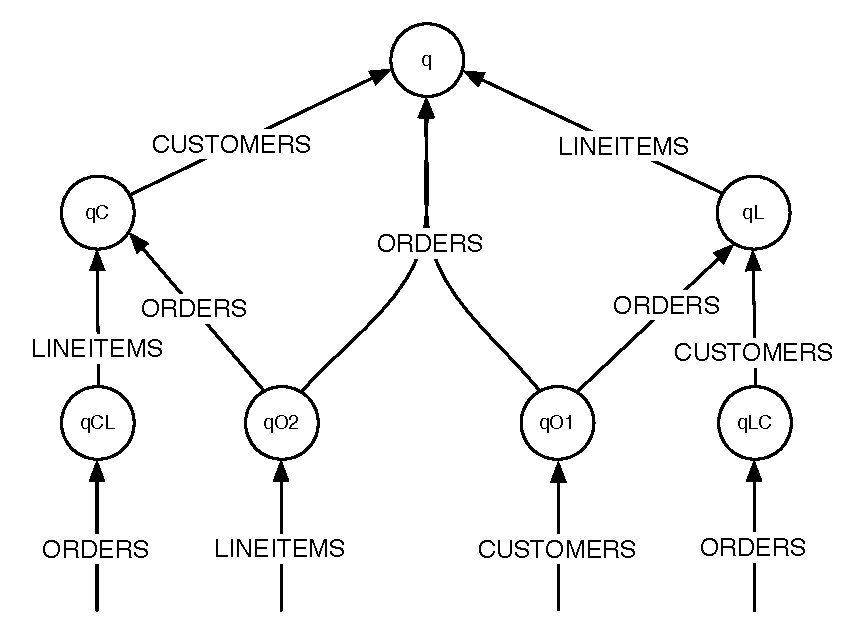
\includegraphics[width=3in]{graphics/q12_graph}
\end{center}
\caption{Dataflow graph for the M3 program representing a streaming TPC-H-style query $\ _{C.cid}G_{SUM(L.price)}(C\ldots \bowtie L\ldots \bowtie O\ldots)$}
\label{fig:dataflow}
\end{figure} 

% Possible TODO: intelligent buffering; How we can stagger buffer periods for a dataflow DAG to limit unfulfilled dependencies down the line.

\subsection{Coordinator Favoritism}

Out of order event processing allows Cumulus to employ decentralized coordinators.  Coordinators are effectively assigned a priority order.  Nodes ensure consistency by consistently evaluating events in the order of their issuing coordinators, regardless of the order in which the events arrive.

This means that lower priority coordinators are much more likely to have unfulfilled dependencies with higher priority coordinators, and thus trigger a cascade.  Worse, the dataflow graphs produced by compiling SQL to M3 are symmetric; there is no assignment of events to coordinators that maps lower priority coordinators to maps further down the dataflow graph.

Cumulus removes this favoritism by staggering each coordinator's epoch transitions.  Each epoch is divided up into a number of periods equal to the number of coordinators.  Each period, the next higher priority coordinator transitions into the next epoch.  This is easily achieved by a token-passing system.  Only the coordinator with the token can switch epochs.  It waits for the duration of one period, switches, and passes the token to the next coordinator.

\subsection{Garbage Collection}
The eventual consistency algorithm uses two datastructures that at first glance appear to be both unbounded and continually growing: The update history, and map values being representated as a list of deltas.  In both cases, the datastructure is unbounded because a value is stored for each version identifier that affects it. 

However, the tail of both datastructures is only needed until updates with earlier version numbers have finished propagating.  The update history is no longer relevant after this point.  Similarly, once version $V$ has finished propagating, prior map entries with earlier versions are used only in the aggregate form.
$$\sum_{V' \leq V} E[V']$$

Thus, it is necessary for the system to be able to discover when all updates have completed propagating through the system.  Cumulus performs this discovery process periodically, once per epoch by default.  

%ABOVE: describe how TCP channels should be used in the section on source aggregation??

Garbage collection occurs in two phases: coordinator synchronization, and node synchronization.  Each coordinator maintains a record of all nodes it sends events to since the last garbage collection.  After a clock-triggered timeout\textit{Coordinators are assumed to have clocks synchronized to within a constant error margin.}, each coordinator begins garbage collecting by sending an \texttt{epoch end} message to all nodes it communicated with.  From this point, the coordinator can begin processing updates for the next epoch.

The following garbage collection process is also illustrated in Figure \ref{fig:GCflowchart}.

\begin{figure}
\begin{center}
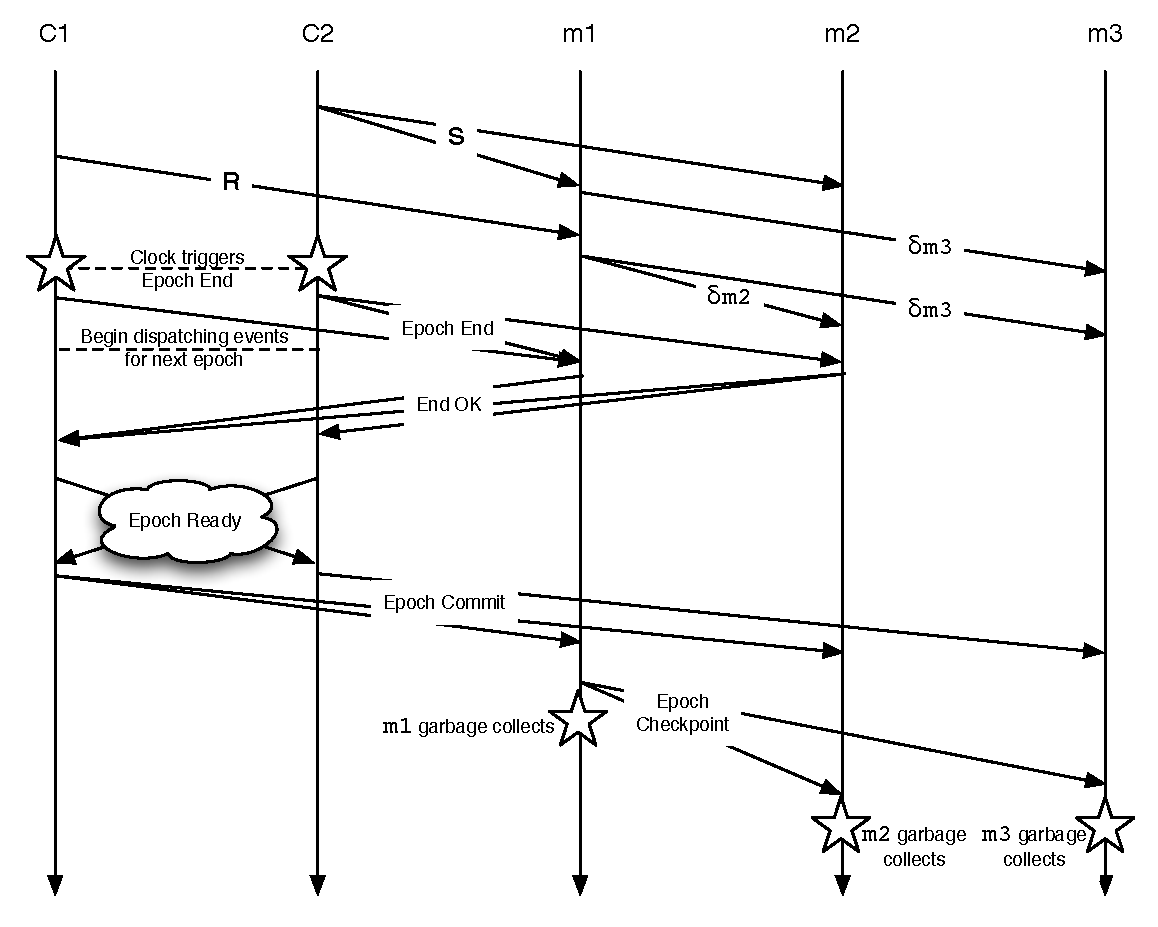
\includegraphics[width=3in]{graphics/GCflowchart}
\caption{Timeline of Garbage Collection for one Epoch in Cumulus; The program being executed is \texttt{ON R() DO \{m1[] += 1; m2[] += m1[]\}; ON S() DO \{m2[] += 1; m3[] += m1[]\}} }
\label{fig:GCflowchart}
\end{center}

%ON R(): m1[] += 1
%        m2[] += m1[]
%ON S(): m2[] += 1
%        m3[] += m1[]
\end{figure}

\begin{figure}
ON Cleanup($V$)
\begin{algorithmic}[1]
\FORALL{Map $M$}
  \FORALL{Entry $E \in M$}
    \STATE $E'[V'] = E[V']$ where $V' > V$
    \STATE $E'[V] = \sum_{V' \leq V} E[V']$
    \STATE replace\_entry($E'$, $M$)
  \ENDFOR
\ENDFOR
\STATE $history =$ filter(delete $history[V']$ if $V' < V$, $history$)
\end{algorithmic}
\caption{Garbage Collection Algorithms}
\label{fig:gcalgorithms}
\end{figure}

Assuming a reliable transport with each message processed in order, when an \texttt{epoch end} from a coordinator, it will have processed and inserted into its history all prior events from that coordinator.  A similar effect can achieved with an unreliable transport.  The node responds to the coordinator with a \texttt{end ok}, confirming that it has processed all of the coordinator's prior messages.  

Once a coordinator receives confirmation from all nodes that it communicated with, it broadcasts an \texttt{epoch ready} message to all other coordinators.  Once all coordinators have sent an \texttt{epoch ready}, the coordinators split the work of broadcasting an \texttt{epoch commit} across the cluster.

Once a node receives an \texttt{epoch commit} message, it will never again receive an event for a prior epoch.  Now, nodes must ensure that no further map deltas will be received.  Using the dataflow graph, a node can determine from where it receives deltas, and to whom it sends deltas.  Because this graph is a DAG in restricted M3, deltas can be flushed along it.  When a node receives an \texttt{epoch commit}, and it sends an \textit{epoch checkpoint} along all of its out edges once after receiving one from all of its in edges.  It then invokes the cleanup process described in Figure \ref{fig:gcalgorithms}.

The act of garbage collection has a very useful added benefit.  In addition to limiting the amount of historical data nodes are required to store, aggregating all deltas prior to a particular version creates a version of the map segment that is consistent with other map segments with the same version across the entire cluster.

\section{Partitioning}
\label{sec:partitioning}

\section{Experiments}

Buffer size vs latency / max throughput.  Intelligent buffering (ie, buffering for greater periods as we go down the dataflow dag)


Eventual+Periodic Consistency.
Subquery computation

{\small
\bibliographystyle{abbrv}
\bibliography{main}
}


\end{document}  